\documentclass[aspectratio=169,dvipsnames]{beamer}

\usetheme{femto}
\setbeamertemplate{section in toc}[ball]

\usepackage[english]{babel}
\usepackage[T1]{fontenc}
\usepackage{xcolor}
\usepackage{adjustbox}
\usepackage{multirow}
\usepackage{nicematrix}
\usepackage{booktabs}
\usepackage{url}
\usepackage{amsmath, amssymb}
\usepackage{centernot}
\usepackage{subcaption}

%
% Check mark and Ballot X
\usepackage{pifont}
\newcommand{\cmark}{{\color{ForestGreen}{\ding{51}}}}
\newcommand{\xmark}{{\color{red}{\ding{55}}}}

%
% Imports tikz and its used libraries.
\usepackage{tikz}
\usetikzlibrary{matrix}
\usetikzlibrary{arrows.meta}
\usetikzlibrary{shapes.arrows}
\usetikzlibrary{pgfplots.groupplots}

%
% Imports libraries for reading csv files and turning them into figures.
\usepackage{pgfplots}
\usepackage{pgfplotstable}
\pgfplotsset{compat=1.18}

\pgfplotstableread[col sep=comma]{./figures/data/dataset_prediction.csv}\PointsPrediction%
\pgfplotstableread[col sep=comma]{./figures/data/dataset_test.csv}\Points%
\pgfplotstableread[col sep=comma]{./figures/data/vertices_convex_0.csv}\ConvexA%
\pgfplotstableread[col sep=comma]{./figures/data/vertices_convex_1.csv}\ConvexB%
\pgfplotstableread[col sep=comma]{./figures/data/vertices_convex_2.csv}\ConvexC%
\pgfplotstableread[col sep=comma]{./figures/data/vertices_convex_3.csv}\ConvexD%
\pgfplotstableread[col sep=comma]{./figures/data/example_rm_limit.csv}\PointsExample%
\pgfplotstableread[col sep=comma]{./figures/data/example_outside_points.csv}\OutsidePoints%
\pgfplotstableread[col sep=comma]{./figures/data/min_max_dataset.csv}\Borders%

%
% Defines global tikz styles for :
% - blue arrows;
% - the ability to hide or show content for slides 
\tikzset{%
	arrowstyle/.style n args=3{%
		single arrow,
		fill=femtogreenstrong,
		anchor=base,
		align=center,
		minimum height=#1,
		single arrow head extend=#2,
		inner sep=#3
	},
	invisible/.style={opacity=0},
	visible on/.style={alt={#1{}{invisible}}},
	alt/.code args={<#1>#2#3}{%
	\alt<#1>{\pgfkeysalso{#2}}{\pgfkeysalso{#3}}
	}
}
\newcommand{\tikzarrow}[3]{%
	\tikz[baseline=-0.5ex]\node[arrowstyle={#1}{#2}{#3}] {};
}


%
% Presentation information.
\title{New convex-based metamorphic relations and large-scale ML model evaluation}
\subtitle{The 37th International Conference on Testing Software and Systems}
\author[Jessy COLONVAL]{\textbf{Jessy COLONVAL\inst{1}} and Fabrice BOUQUET\inst{1}}
\institute{%
	\inst{1} Université Marie et Louis Pasteur, CNRS, insitut FEMTO-ST (UMR 6174), F-25000 Besançon, France
}
\date{17 September 2025}


\begin{document}

% Colors used for test tables.
\definecolor{CustomRed}{HTML}{FF6666}%FFACAB}
\definecolor{CustomLightRed}{HTML}{FEDBD5}
\definecolor{CustomOrange}{HTML}{FFD7B3}
\definecolor{CustomYellow}{HTML}{FFF6BA}
\definecolor{CustomLightGreen}{HTML}{EEFADB}
\colorlet{CustomGreen}{SpringGreen!80}


%%% Macro that defines colors according to test success.
%%%%%%%%%%%%%%%%%%%%%%%%%%%%%%%%%%%%%%%%%%%%%%%%%%%%%%%%%%%%%%%%%%%%%%%%%%%%%%%%%%%%%%%%%%
% PassedTest        |      Vert (CustomGreen)                  | = 100%
% OftenPassedTest   |      Vert clair (CustomLightGreen)       | 75 >= and < 100
% EvenPassedTest    |      Jaune (CustomYellow)                | 50 >= and < 75
% OftenFailedTest   |      Orange (CustomOrange)               | 25 >= and < 50
% TooManyFailedTest |      Rouge clair (CustomLightRed)        | 0 > and < 25
% FailedTest        |      Rouge (CustomRed)                   | = 0 %
%%%%%%%%%%%%%%%%%%%%%%%%%%%%%%%%%%%%%%%%%%%%%%%%%%%%%%%%%%%%%%%%%%%%%%%%%%%%%%%%%%%%%%%%%%
\newcommand{\PassedTest}[0]{\cellcolor{CustomGreen}}
\newcommand{\FailedTest}[0]{\cellcolor{CustomRed}}
\newcommand{\TooManyFailedTest}[0]{\cellcolor{CustomLightRed}}
\newcommand{\OftenFailedTest}[0]{\cellcolor{CustomOrange}}
\newcommand{\EvenPassedTest}[0]{\cellcolor{CustomYellow}}
\newcommand{\OftenPassedTest}[0]{\cellcolor{CustomLightGreen}}

\newcolumntype{M}[1]{>{\centering\arraybackslash}m{#1}}


\begin{frame}[plain, c]
	\titlepage%
\end{frame}

\begin{frame}{Table of contents}
	\tableofcontents
\end{frame}

\section{Context}

\begin{frame}{\secname}
	\framesubtitle{Oracle problem}
	Oracle hypothesis: it's possible to determine if an output is correct\\
	\tikzarrow{0.75cm}{0.15cm}{0.1cm}FALSE
	\pause%

	\vspace{\baselineskip}
	In reality:
	\begin{itemize}
		\item no oracle;
		\item too difficult too implement.
	\end{itemize}
	\pause%

	\vspace{\baselineskip}
	\textbf{Machine learning models have an oracle problem!}
\end{frame}

\begin{frame}{\secname}
	\framesubtitle{Oracle problem}
	Metamorphic relations:
	\begin{itemize}
		\item No verification of each input / output;
		\item Verification of properties between input / output.
	\end{itemize}

	\vspace{\baselineskip}
	\tikzarrow{0.75cm}{0.15cm}{0.1cm}\textbf{Ligthen the problem of the oracle!}
\end{frame}


\section{State-of-the-art metamorphic relations}

\begin{frame}{Table of contents}
	\tableofcontents[currentsection]
\end{frame}

\begin{frame}{\secname}
	\framesubtitle{Identity relation --- MR~1}
	When two models have the same:
	\begin{itemize}
		\item training algorithm;
		\item meta-parameters;
		\item data sets.
	\end{itemize}
	\pause%

	\vspace{\baselineskip}
	\tikzarrow{0.75cm}{0.15cm}{0.1cm}\textbf{Outputs must be identical!}
\end{frame}

\begin{frame}{\secname}
	\framesubtitle{Points shuffle relation --- MR~2}
	\begin{figure}
        	\centering
        	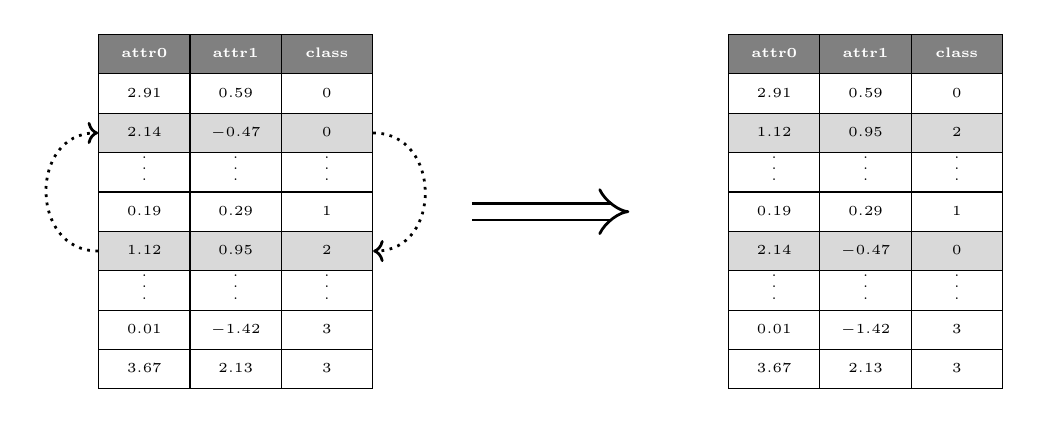
\begin{tikzpicture}
			\tiny
			\matrix[%
				matrix of nodes,
				row sep=-\pgflinewidth, column sep=-\pgflinewidth,
				nodes={draw, fill=white, text centered, text width=1cm,
				minimum height=5mm, text height=1.5ex, text depth=.25ex, anchor=center},
				row 1/.style={nodes={fill=gray, text=white}},
				row 4/.style={nodes={text depth=0cm, text height=2.9ex}},
				row 7/.style={nodes={text depth=0cm, text height=2.9ex}},
	           		row 3/.style={nodes={fill=gray!30}},
        	                row 6/.style={nodes={fill=gray!30}},
                	        ampersand replacement=\&
			]
	                (original) at (-4, 0) {%
	                	\textbf{attr0} \& \textbf{attr1} \& \textbf{class} \\
		                $2.91$ \& $0.59$ \& $0$ \\ 
        		        $2.14$ \& $-0.47$ \& $0$ \\
                		\vdots \& \vdots \& \vdots \\
		                $0.19$ \& $0.29$ \& $1$ \\
        		        $1.12$ \& $0.95$ \& $2$ \\
                		\vdots \& \vdots \& \vdots \\
	                	$0.01$ \& $-1.42$ \& $3$ \\
	        	        $3.67$ \& $2.13$ \& $3$ \\
            		};

	                \matrix[%
        	        	matrix of nodes,
	                	row sep=-\pgflinewidth, column sep=-\pgflinewidth,
        	        	standard size/.style={minimum height=4mm, text width=1cm},
                		nodes={draw, fill=white, text centered, text width=1cm,
		                minimum height=5mm, text height=1.5ex, text depth=.25ex, anchor=center},
        		        row 1/.style={nodes={fill=gray, text=white}},
                		row 4/.style={nodes={text depth=0cm, text height=2.9ex}},
		                row 7/.style={nodes={text depth=0cm, text height=2.9ex}},
        	        	row 3/.style={nodes={fill=gray!30}},
        	        	row 6/.style={nodes={fill=gray!30}},
	        	        ampersand replacement=\&
        	    	]
	            	(transformed) at (4, 0) {%
				\textbf{attr0} \& \textbf{attr1} \& \textbf{class} \\
		                $2.91$ \& $0.59$ \& $0$ \\
        		        $1.12$ \& $0.95$ \& $2$ \\
                		\vdots \& \vdots \& \vdots \\
	                	$0.19$ \& $0.29$ \& $1$ \\
	        	        $2.14$ \& $-0.47$ \& $0$ \\
        	        	\vdots \& \vdots \& \vdots \\
	        	        $0.01$ \& $-1.42$ \& $3$ \\
        	        	$3.67$ \& $2.13$ \& $3$ \\
            		};

	                \draw[dotted, ->, line width=1pt] (original-3-3.east) to[out=0, in=0, looseness=1.5] (original-6-3.east);
                 	\draw[dotted, ->, line width=1pt] (original-6-1.west) to[out=180,in=180,looseness=1.5](original-3-1.west);

	                \draw[-Implies, line width=1pt, double distance=5pt] (-1,0) to (1,0);
		\end{tikzpicture}
	\end{figure}
	\pause%

	\tikzarrow{0.75cm}{0.15cm}{0.1cm}\textbf{Outputs must be identical!}\\
	\hspace{0.85cm}{\color{BrickRed}\textbf{Except when part of points are used.}}
\end{frame}

\begin{frame}{\secname}
	\framesubtitle{Attributes shuffle --- MR~3}
	\begin{figure}
		\centering
		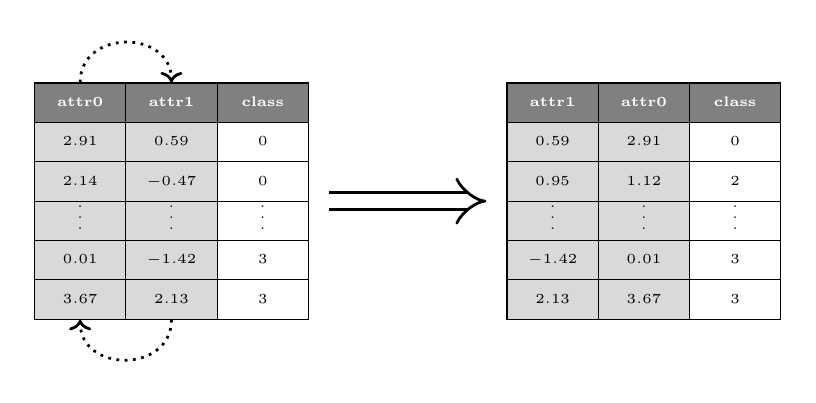
\begin{tikzpicture}
			\tiny
			\matrix[%
				matrix of nodes,
				row sep=-\pgflinewidth, column sep=-\pgflinewidth,
				nodes={draw, fill=white, text centered, text width=1cm,
				minimum height=5mm, text height=1.5ex, text depth=.25ex, anchor=center},
				row 1/.style={nodes={fill=gray, text=white}},
				row 4/.style={nodes={text depth=0cm, text height=2.9ex}},
				column 1/.style={nodes={fill=gray!30}},
				column 2/.style={nodes={fill=gray!30}},
				ampersand replacement=\&
			]
			(original) at (-3,0) {%
				\textbf{attr0} \& \textbf{attr1} \& \textbf{class} \\
				$2.91$ \& $0.59$ \& $0$ \\
				$2.14$ \& $-0.47$ \& $0$ \\
				\vdots \& \vdots \& \vdots \\
				$0.01$ \& $-1.42$ \& $3$ \\
				$3.67$ \& $2.13$ \& $3$ \\
			};

			\matrix[%
				matrix of nodes,
				row sep=-\pgflinewidth, column sep=-\pgflinewidth,
				nodes={draw, fill=white, text centered, text width=1cm,
					minimum height=5mm, text height=1.5ex, text depth=.25ex, anchor=center},
				row 1/.style={nodes={fill=gray, text=white}},
				row 4/.style={nodes={text depth=0cm, text height=2.9ex}},
				column 1/.style={nodes={fill=gray!30}},
				column 2/.style={nodes={fill=gray!30}},
				ampersand replacement=\&
			]
			(transformed) at (3,0) {%
				\textbf{attr1}\&\textbf{attr0}\&\textbf{class}\\
				$0.59$ \& $2.91$ \& $0$ \\
				$0.95$ \& $1.12$ \& $2$ \\
				\vdots \& \vdots \& \vdots \\
				$-1.42$ \& $0.01$ \& $3$ \\
				$2.13$ \& $3.67$ \& $3$ \\
			};

			\draw[dotted,->, line width=1pt] (original-1-1.north) to [out=90, in=90, looseness=1.5] (original-1-2.north);
			\draw[dotted,->, line width=1pt] (original-6-2.south) to [out=-90, in=-90, looseness=1.5] (original-6-1.south);

			\draw[-Implies, line width=1pt, double distance=5pt] (-1,0) to (1,0);
		\end{tikzpicture}
	\end{figure}
	\pause%

	\tikzarrow{0.75cm}{0.15cm}{0.1cm}\textbf{Outputs must be identical!}\\
	\hspace{0.85cm}{\color{BrickRed}\textbf{Except when part of attributes are used.}}
\end{frame}

\begin{frame}{\secname}
	\framesubtitle{Transformation relation --- MR~4}
	\begin{figure}
		\centering
		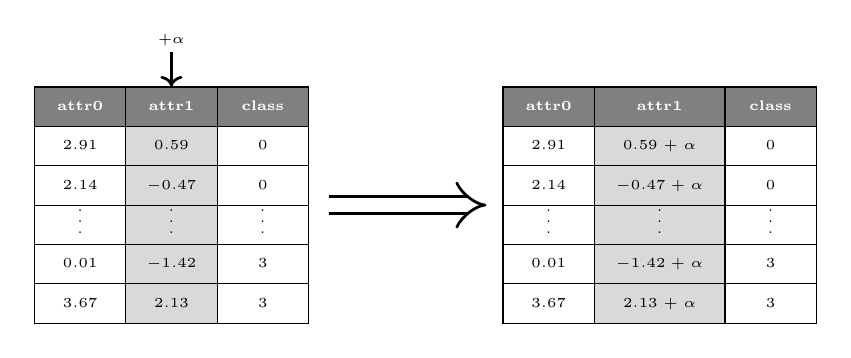
\begin{tikzpicture}
			\tiny
			\matrix[%
				matrix of nodes,
				row sep=-\pgflinewidth, column sep=-\pgflinewidth,
				nodes={draw, fill=white, text centered, text width=1cm,
				minimum height=5mm, text height=1.5ex, text depth=.25ex, anchor=center},
				row 1/.style={nodes={fill=gray, text=white}},
				row 4/.style={nodes={text depth=0cm, text height=2.9ex}},
				column 2/.style={nodes={fill=gray!30}},
				ampersand replacement=\&
			]
			(original) at (-3, 0) {%
				\textbf{attr0} \& \textbf{attr1} \& \textbf{class} \\
				$2.91$ \& $0.59$ \& $0$ \\ 
				$2.14$ \& $-0.47$ \& $0$ \\
				\vdots \& \vdots \& \vdots \\
				$0.01$ \& $-1.42$ \& $3$ \\
				$3.67$ \& $2.13$ \& $3$ \\
			};

			\matrix[%
				matrix of nodes,
				row sep=-\pgflinewidth, column sep=-\pgflinewidth,
				nodes={draw, fill=white, text centered, text width=1cm,
				minimum height=5mm, text height=1.5ex, text depth=.25ex, anchor=center},
				row 1/.style={nodes={fill=gray, text=white}},
				row 4/.style={nodes={text depth=0cm, text height=2.9ex}},
				column 2/.style={nodes={fill=gray!30, text width=1.5cm}},
				ampersand replacement=\&
			]
			(transformed) at (3.2, 0) {%
				\textbf{attr0} \& \textbf{attr1} \& \textbf{class} \\
				$2.91$ \& $0.59 + \alpha$ \& $0$ \\ 
				$2.14$ \& $-0.47 + \alpha$ \& $0$ \\
				\vdots \& \vdots \& \vdots \\
				$0.01$ \& $-1.42 + \alpha$ \& $3$ \\
				$3.67$ \& $2.13 + \alpha$ \& $3$ \\
			};

			\node at (-3, 2.1) (plus) {$+\alpha$};
			\draw[->, line width=1pt] (plus.south) to (original-1-2.north);

			\draw[-Implies, line width=1pt, double distance=5pt] (-1,0) to (1,0);
		\end{tikzpicture}
	\end{figure}
	\pause%

	\tikzarrow{0.75cm}{0.15cm}{0.1cm}\textbf{Outputs must be identical!}
\end{frame}

\begin{frame}{\secname}
	\framesubtitle{Class permutation relation --- MR~5}
	\begin{figure}
		\centering
		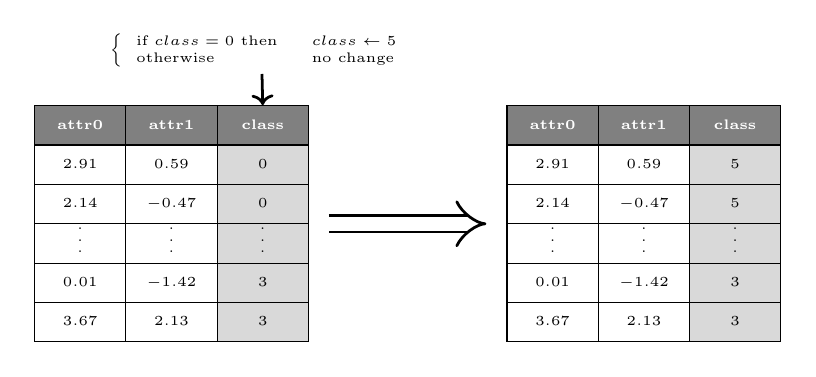
\begin{tikzpicture}
			\tiny
			\matrix[%
				matrix of nodes,
				row sep=-\pgflinewidth, column sep=-\pgflinewidth,
				nodes={draw, fill=white, text centered, text width=1cm,
				minimum height=5mm, text height=1.5ex, text depth=.25ex, anchor=center},
				row 1/.style={nodes={fill=gray, text=white}},
				row 4/.style={nodes={text depth=0cm, text height=2.9ex}},
				column 3/.style={nodes={fill=gray!30}},
				ampersand replacement=\&
			]
			(original) at (-3, 0) {%
				\textbf{attr0} \& \textbf{attr1} \& \textbf{class} \\
				$2.91$ \& $0.59$ \& $0$ \\ 
				$2.14$ \& $-0.47$ \& $0$ \\
				\vdots \& \vdots \& \vdots \\
				$0.01$ \& $-1.42$ \& $3$ \\
				$3.67$ \& $2.13$ \& $3$ \\
			};

			\matrix[%
				matrix of nodes,
				row sep=-\pgflinewidth, column sep=-\pgflinewidth,
				nodes={draw, fill=white, text centered, text width=1cm,
				minimum height=5mm, text height=1.5ex, text depth=.25ex, anchor=center},
				row 1/.style={nodes={fill=gray, text=white}},
				row 4/.style={nodes={text depth=0cm, text height=2.9ex}},
				column 3/.style={nodes={fill=gray!30}},
				ampersand replacement=\&
			]
			(transformed) at (3, 0) {%
				\textbf{attr0} \& \textbf{attr1} \& \textbf{class} \\
				$2.91$ \& $0.59$ \& $5$ \\ 
				$2.14$ \& $-0.47$ \& $5$ \\
				\vdots \& \vdots \& \vdots \\
				$0.01$ \& $-1.42$ \& $3$ \\
				$3.67$ \& $2.13$ \& $3$ \\
			};

			\node at (-1.85, 2.2)   (modif) {$\left \{\begin{array}{ll}\text{if } class = 0 \text{ then }  & class \leftarrow 5\\\text{otherwise} & \text{no change} \\\end{array}\right .$};
			\draw[->, line width=1pt] (modif.south) to (original-1-3.north);

			\draw[-Implies, line width=1pt, double distance=5pt] (-1,0) to (1,0);
		\end{tikzpicture}
	\end{figure}
	\pause%

	\tikzarrow{0.75cm}{0.15cm}{0.1cm}\textbf{Outputs must be identical!}
\end{frame}


\section{Convex-based metamorphic relations}

\begin{frame}{Table of contents}
	\tableofcontents[currentsection]
\end{frame}

\begin{frame}{\secname}
	\framesubtitle{Convex definition}

	\begin{definition}
		A part $H$ of $\mathbb{R}^{n}$ said to be convex if, for all pairs $(x,y)$ of elements of $H$, the segment $[x,y]$ is entirely contained within $H$.
		In other words, $H$ is convex when $\forall x,y \in H$ and $\forall \lambda \in [0;1], \lambda x + (1-\lambda)y \in H$~[10].
	\end{definition}

	\begin{figure}[H]
		\centering
		\begin{subfigure}{0.45\textwidth}
			\centering
			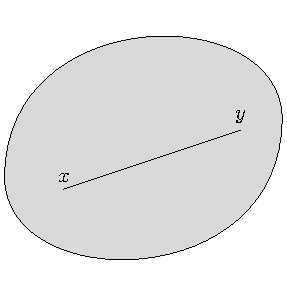
\includegraphics[width=0.5\textwidth]{./figures/example_convex}
			\caption{A convex}
		\end{subfigure}
		\hfill
		\begin{subfigure}{0.45\textwidth}
			\centering
			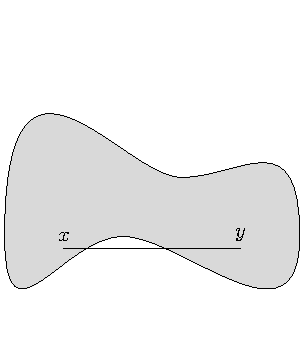
\includegraphics[width=0.5\textwidth]{./figures/example_non_convex}
			\caption{A non-convex}
		\end{subfigure}
	\end{figure}
\end{frame}

\begin{frame}{\secname}
	\framesubtitle{How they are created?}

	\begin{itemize}
		\item Using the algorithm \textbf{QuickHull} $n$D (\textit{QHull}\footnote{\url{http://www.qhull.org/}}).
		\item Approximation of influence areas of classes.
	\end{itemize}

	\begin{figure}[H]
		\centering
		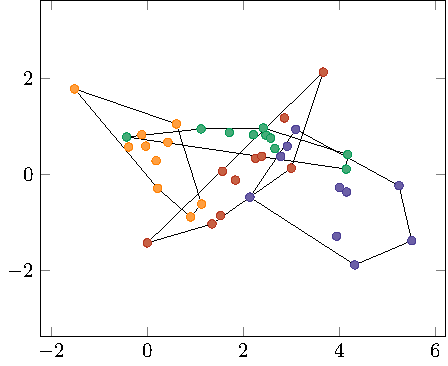
\includegraphics[width=0.4\textwidth]{./figures/dataset_presentation}
	\end{figure}
\end{frame}

\begin{frame}{\secname}
	\framesubtitle{Membership relation --- MR~6}
	Hypothesis:
	\begin{itemize}
		\item Convex = one area of class.
		\item Point inside \tikzarrow{0.75cm}{0.15cm}{0.1cm}similar characteristics.
	\end{itemize}
	\hspace{2.847cm}\tikzarrow{0.75cm}{0.15cm}{0.1cm}identical class.

	\begin{figure}[H]
		\centering
		\vspace{-1cm}
		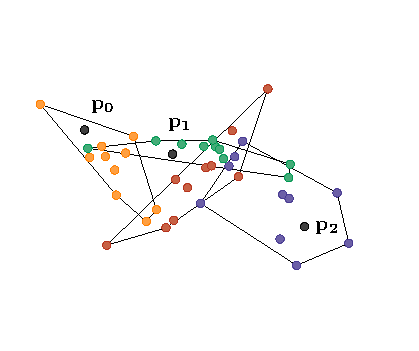
\includegraphics{./figures/example_appartenance}
	\end{figure}
\end{frame}

\begin{frame}{\secname}
	\framesubtitle{Superposition relation --- MR~7}
	Observations:
	\begin{itemize}
		\item Shared areas.
		\item Which choice will the models make? \tikzarrow{0.75cm}{0.15cm}{0.1cm}We don't choose!
	\end{itemize}

	\begin{figure}[H]
		\centering
		\vspace{-1cm}
		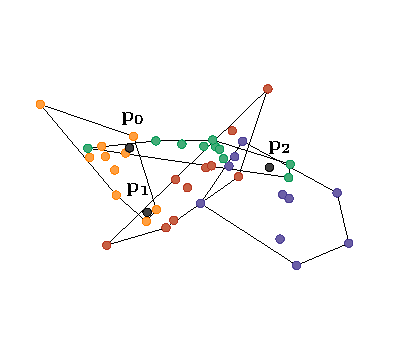
\includegraphics{./figures/example_superposition}
	\end{figure}
\end{frame}

\begin{frame}{\secname}
	\framesubtitle{Attachment relation --- MR~8}
	Hypothesis:
	\begin{itemize}
		\item Model extrapolation.
		\item Nearest convex(es) \tikzarrow{0.75cm}{0.15cm}{0.1cm}similar characteristics.
	\end{itemize}
	\hspace{4.183cm}\tikzarrow{0.75cm}{0.15cm}{0.1cm}identical class.

	\begin{figure}[H]
		\centering
		\vspace{-1cm}
		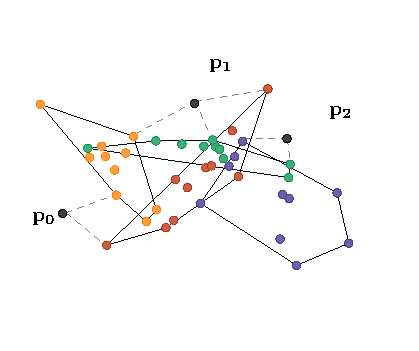
\includegraphics{./figures/example_rattachement}
	\end{figure}
\end{frame}

\begin{frame}{\secname}
	\framesubtitle{Limits \& Robustness}

	\begin{minipage}{0.5\textwidth}
		Tests evaluate values:
		\begin{itemize}
			\item within the limits;
	            	\item at the limits;
            		\item off limits.
        	\end{itemize}
    	\end{minipage}%
	\begin{minipage}{0.8\textwidth}
        	\pause%
	        \vspace{\baselineskip}
        	\vspace{\itemsep}
	        \hspace{-1.5cm}\tikzarrow{0.75cm}{0.15cm}{0.1cm}in the domain;
        	\vspace{\itemsep}

	        \hspace{-1.5cm}\tikzarrow{0.75cm}{0.15cm}{0.1cm}borders of the domain;
        	\vspace{\itemsep}

	        \hspace{-1.5cm}\tikzarrow{0.75cm}{0.15cm}{0.1cm}outside the domain.
	\end{minipage}

	\pause%
	\vspace{\baselineskip}
	Models must:
    	\vspace{\itemsep}

	\tikzarrow{0.75cm}{0.15cm}{0.1cm} Do not produce an error: \textbf{Robustness --- MR~9}
   	\vspace{\itemsep}

	\tikzarrow{0.75cm}{0.15cm}{0.1cm} Do not produce an error when the value is outside the domain: \textbf{Boundary Robustness --- MR~10}
   	\vspace{\itemsep}

	\tikzarrow{0.75cm}{0.15cm}{0.1cm} Respect the relation \textbf{Boundary Attachment --- MR~11}
\end{frame}

\begin{frame}{\secname}
	\framesubtitle{Illustration of the use of limits}

    	\begin{minipage}{0.65\textwidth}
    		\begin{figure}[H]
        		\centering
        		\begin{tikzpicture}
            			%%%%%%%%%%%%% Generated points's labels. %%%%%%%%%%%%%
            			% Angles.
			        \node[visible on=<1->] at (0.74, 4.4) {$\mathbf{p_{0}}$};
            			\node[visible on=<1->] at (5.59, 4.4) {$\mathbf{p_{1}}$};
            			\node[visible on=<1->] at (0.74, 1.0) {$\mathbf{p_{2}}$};
            			\node[visible on=<1->] at (5.59, 1.0) {$\mathbf{p_{3}}$};
            			% On borders.
            			\node[visible on=<2->] at (0.1, 2.8) {$\mathbf{p_{4}}$};
            			\node[visible on=<2->] at (2.7, 1.0) {$\mathbf{p_{5}}$};
            			\node[visible on=<2->] at (3.8, 4.4) {$\mathbf{p_{6}}$};
            			\node[visible on=<2->] at (6.1, 2.8) {$\mathbf{p_{7}}$};
            			% Outside borders.
            			\node[visible on=<3->] at (-0.25, 2.1) {$\mathbf{p'_{0}}$};
            			\node[visible on=<3->] at (4.1, 0.8) {$\mathbf{p'_{1}}$};
            			\node[visible on=<3->] at (2.1, 4.7) {$\mathbf{p'_{2}}$};
            			\node[visible on=<3->] at (7.15, 3.5) {$\mathbf{p'_{3}}$};

            			% Convexes.
            			\begin{axis}[%
                			axis equal,
                			scatter/classes={%
                    				{0}={draw=BlueViolet, fill=BlueViolet!75},
                    				{1}={draw=orange, fill=orange!75},
                    				{2}={draw=ForestGreen, fill=ForestGreen!75},
                    				{3}={draw=BrickRed, fill=BrickRed!75},
                    				{-1}={draw=black, fill=black!75}
                			},
                			axis line style={draw=none},
                			tick style={draw=none},
                			xticklabel=\empty, yticklabel=\empty,
                			xmin=-2.1, xmax=7.1,
                			ymin=-2.14, ymax=2.78
            			]
                			\addplot[scatter, only marks, scatter src=explicit symbolic, mark size=1.43pt, visible on=<1->] table [x={attr0}, y={attr1}, meta={class}, col sep=comma] {\Points};
                			\addplot[scatter, scatter src=explicit symbolic, mark size=1.43pt] table [x={attr0}, y={attr1}, meta={class}, col sep=comma, visible on=<1->] {\ConvexA};
                			\addplot[scatter, scatter src=explicit symbolic, mark size=1.43pt] table [x={attr0}, y={attr1}, meta={class}, col sep=comma, visible on=<1->] {\ConvexB};
                			\addplot[scatter, scatter src=explicit symbolic, mark size=1.43pt] table [x={attr0}, y={attr1}, meta={class}, col sep=comma, visible on=<1->] {\ConvexC};
                			\addplot[scatter, scatter src=explicit symbolic, mark size=1.43pt] table [x={attr0}, y={attr1}, meta={class}, col sep=comma, visible on=<1->] {\ConvexD};
                			\addplot[dashed, scatter, scatter src=explicit symbolic, mark size=1.43pt] table [x={attr0}, y={attr1}, meta={class}, col sep=comma, visible on=<2->] {\Borders};
                			\addplot[scatter, only marks, scatter src=explicit symbolic, mark size=1.43pt, visible on=<2->] table [x={attr0}, y={attr1}, meta={class}, col sep=comma] {\PointsExample};
                			\addplot[scatter, only marks, scatter src=explicit symbolic, mark size=1.43pt, visible on=<3->] table [x={attr0}, y={attr1}, meta={class}, col sep=comma] {\OutsidePoints};
            			\end{axis}
        		\end{tikzpicture}
    		\end{figure}
    	\end{minipage}%
    	\begin{minipage}{0.35\textwidth}
        	\textbf{Values}:
        	\begin{itemize}
            		\item all at the limits;
            		\pause%
            		\item only one at the limits;
            		\pause%
            		\item one out of limits.
        	\end{itemize}
    	\end{minipage}
\end{frame}


\section{Non-convex metamorphic relations}

\begin{frame}{Table of contents}
	\tableofcontents[currentsection]
\end{frame}

\begin{frame}{\secname}
	\framesubtitle{Precision relation --- MR~12}

	\begin{figure}
		\centering
		\begin{subfigure}{0.48\textwidth}
			\centering
			\begin{tikzpicture}
				\begin{axis}[%
					axis line style={draw=none},
					tick style={draw=none},
					xticklabel=\empty, yticklabel=\empty,
					scatter/classes={%
						{0}={draw=BlueViolet, fill=BlueViolet!50},
						{1}={draw=orange, fill=orange!50},
						{2}={draw=ForestGreen, fill=ForestGreen!50},
						{3}={draw=BrickRed, fill=BrickRed!50}
					},
					xmin=-8, xmax=8,
					ymin=-5, ymax=5
				]
					\addplot[scatter, only marks, scatter src=explicit symbolic] table [x={attr0}, y={attr1}, meta={class}, col sep=comma] {\PointsPrediction};
					\draw[->,ultra thick] (-7,0)--(7,0) node[right] {$x$};
					\draw[->,ultra thick] (0,-4)--(0,4) node[above] {$y$};
					\draw[red] (7,4)--(-7,-4);
					\draw[red] (7,-4)--(-7,4);
				\end{axis}
			\end{tikzpicture}
			\caption{Data set}
		\end{subfigure}
		\hfill
		\begin{subfigure}{0.48\textwidth}
			\centering
			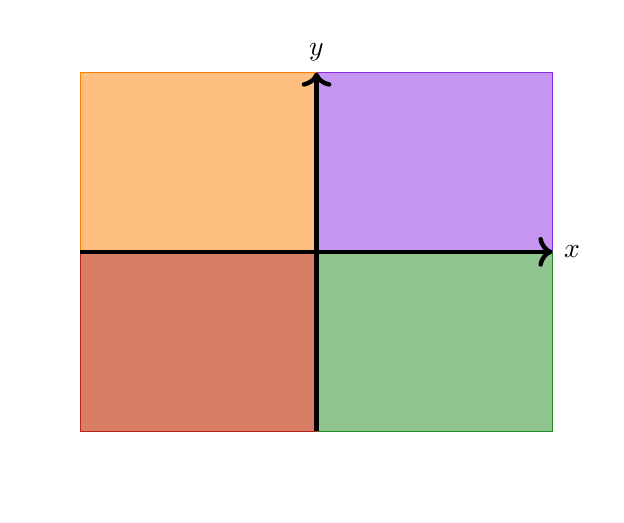
\begin{tikzpicture}
				\begin{axis}[%
					axis line style={draw=none},
					tick style={draw=none},
					xticklabel=\empty, yticklabel=\empty,
					scatter/classes={%
						{0}={draw=BlueViolet, fill=BlueViolet},
						{1}={draw=orange, fill=orange},
						{2}={draw=ForestGreen, fill=ForestGreen},
						{3}={draw=BrickRed, fill=BrickRed}
					},
					xmin=-8, xmax=8,
					ymin=-5, ymax=5
				]
					\draw[draw = BlueViolet, fill = BlueViolet!50] (0,4) rectangle (7,0);
					\draw[draw = orange, fill = orange!50] (-7,4) rectangle (0,0);
					\draw[draw = ForestGreen, fill = ForestGreen!50] (0,0) rectangle (7,-4);
					\draw[draw = BrickRed, fill = BrickRed!50] (-7,-4) rectangle (0,0);

					\draw[->,ultra thick] (-7,0)--(7,0) node[right]{$x$};
					\draw[->,ultra thick] (0,-4)--(0,4) node[above]{$y$};
				\end{axis}
			\end{tikzpicture}
			\caption{Expected predictions}
		\end{subfigure}
	\end{figure}
\end{frame}

\begin{frame}{\secname}
	\framesubtitle{Outliers relation --- MR~13}

	\begin{minipage}{0.65\textwidth}
		\begin{figure}
			\centering
			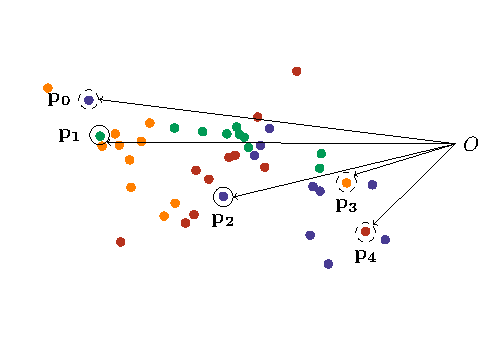
\includegraphics{./figures/example_outliers}
		\end{figure}
	\end{minipage}%
	\begin{minipage}{0.35\textwidth}
		Origin:
		\begin{itemize}
			\item added to the dataset;
			\item already existing.
		\end{itemize}
	\end{minipage}
	\pause%

	\tikzarrow{0.75cm}{0.15cm}{0.1cm}\textbf{Models shoudn't predict them correctly!}
\end{frame}

\section{Experimentations}

\begin{frame}{Table of contents}
	\tableofcontents[currentsection]
\end{frame}

\begin{frame}{\secname}
	\framesubtitle{Synthetic data sets}

	\begin{adjustbox}{max height=0.75\textheight, center}
		\begin{NiceTabular}{|l|l|c|l|c|c|}
			\hline
			\textbf{Points} & \textbf{Attributes} & \textbf{Classes} & \textbf{Noises} & \textbf{Distribution} & \textbf{Ratio} \\
			\hline
			$\mathbf{s}$ -- $250$ & $\mathbf{s}$ -- $10$ & $\mathbf{b}$& $\mathbf{n}$ & $\mathbf{ho}$ & $\mathbf{y}$ \\
			$\mathbf{s}$ -- $250$ & $\mathbf{m}$ -- $100$ & $\mathbf{p}$ -- $5$ & $\mathbf{y}$ - $60\%$ & $\mathbf{he}$ & $\mathbf{n}$ \\
			$\mathbf{s}$ -- $250$ & $\mathbf{l}$ -- $1\,000$ & $\mathbf{b}$ & $\mathbf{y}$ -- $10\%$ & $\mathbf{ho}$ & $\mathbf{n}$ \\
			$\mathbf{m}$ -- $25\,000$ & $\mathbf{s}$ -- $10$ & $\mathbf{b}$ & $\mathbf{y}$ -- $60\%$ & $\mathbf{he}$ & $\mathbf{y}$ \\
			$\mathbf{m}$ -- $25\,000$ & $\mathbf{m}$ -- $100$ & $\mathbf{p}$ -- $5$ & $\mathbf{y}$ -- $10\%$ & $\mathbf{ho}$ & $\mathbf{y}$ \\
			$\mathbf{m}$ -- $25\,000$ & $\mathbf{l}$ -- $1\,000$ & $\mathbf{b}$ & $\mathbf{n}$ & $\mathbf{he}$ & $\mathbf{y}$ \\
			$\mathbf{l}$ -- $125\,000$ & $\mathbf{s}$ -- $10$ & $\mathbf{p}$ -- $5$ & $\mathbf{y}$ -- $10\%$ & $\mathbf{he}$ & $\mathbf{y}$ \\
			$\mathbf{l}$ -- $125\,000$ & $\mathbf{m}$ -- $100$ & $\mathbf{b}$ & $\mathbf{y}$ -- $60\%$ & $\mathbf{ho}$ & $\mathbf{y}$ \\
			$\mathbf{l}$ -- $125\,000$ & $\mathbf{m}$ -- $100$ & $\mathbf{b}$ & $\mathbf{n}$ & $\mathbf{ho}$ & $\mathbf{y}$ \\
			\hline
		\end{NiceTabular}
	\end{adjustbox}
\end{frame}

\begin{frame}{\secname}
	\framesubtitle{Algorithms}

	\begin{minipage}{0.5\textwidth}
	\begin{adjustbox}{max height=0.4\textheight, center}
		\begin{NiceTabular}{lccccc}
			\CodeBefore
				% Decision Tree
				\cellcolor{gray!50}{6-2}
				% Extra Tree
				\cellcolor{gray!50}{7-2}
				% Random Forest
				\cellcolor{gray!50}{20-2}
				% Dummy
				\cellcolor{gray!50}{8-4}
				% Gaussian
				\cellcolor{gray!50}{9-3}
				% Passive Agressive
				\cellcolor{gray!50}{16-3}
				% Ridge
				\cellcolor{gray!50}{21-3}
				% SGD
				\cellcolor{gray!50}{22-3}
				% Bernouli
				\cellcolor{gray!50}{3-2}
				\cellcolor{gray!50}{3-5}
				% Categorical
				\cellcolor{gray!50}{4-2}
				\cellcolor{gray!50}{4-5}
				% Complement
				\cellcolor{gray!50}{5-2}
				\cellcolor{gray!50}{5-5}
				% Multinominal
				\cellcolor{gray!50}{14-2}
				\cellcolor{gray!50}{14-5}
				% KNN
				\cellcolor{gray!50}{11-6}
				% Radius neighbors
				\cellcolor{gray!50}{19-6}
				% MLP
				\cellcolor{gray!50}{13-5}
				% SVC
				\cellcolor{gray!50}{23-3}
				% Linear
				\cellcolor{gray!50}{12-3}
				% Quadratic
				\cellcolor{gray!50}{18-3}
				% Gradient
				\cellcolor{gray!50}{10-2}
				% Perceptron
				\cellcolor{gray!50}{17-5}
				% Nearest Centroid
				\cellcolor{gray!50}{15-6}
			\Body
				& \multicolumn{5}{c}{\textbf{Paradigm}} \\
				& \textbf{(1)} & \textbf{(2)} & \textbf{(3)} & \textbf{(4)} & \textbf{(5)} \\
				\midrule
				\textit{Bernoulli NB}&&&&&\\
				\textit{Categorical NB}&&&&&\\
				\textit{Complement NB}&&&&&\\
				\textit{Decision Tree Classifier}&&&&&\\
				\textit{Extra Tree Classifier}&&&&&\\
				\textit{Dummy Classifier}&&&&&\\
				\textit{Gaussian Process Classifier}&&&&&\\
				\textit{Gradient Boosting Classifier} &&&&&\\
				\textit{K Neighbors Classifier}&&&&&\\
				\textit{Linear Discriminant Analysis}&&&&&\\
				\textit{MLP Classifier}&&&&&\\
				\textit{Multinomial NB}&&&&&\\
				\textit{Nearest Centroid}&&&&&\\
				\textit{Passive Aggressive Classifier}&&&&&\\
				\textit{Perceptron}&&&&&\\
				\textit{Quadratic Distriminant Analysis}~&&&&&\\
				\textit{Radius Neighbors Classifier}&&&&&\\
				\textit{Random Forest Classifier}&&&&&\\
				\textit{Ridge Classifier}&&&&&\\
				\textit{SGD Classifier}&&&&&\\
				\textit{SVC}&&&&&\\
				\bottomrule
			\CodeAfter
				\begin{tikzpicture}
					\draw (1-|2) -- (1-|7) ;
					%
					\draw (1-|2) -- (24-|2) ;
					\draw (3-|3) -- (24-|3) ;
					\draw (3-|4) -- (24-|4) ;
					\draw (3-|5) -- (24-|5) ;
					\draw (3-|6) -- (24-|6) ;
					\draw (1-|7) -- (24-|7) ;
					%
					\draw[dotted] (4-|1) -- (4-|7) ;
					\draw[dotted] (5-|1) -- (5-|7) ;
					\draw[dotted] (6-|1) -- (6-|7) ;
					\draw[dotted] (7-|1) -- (7-|7) ;
					\draw[dotted] (8-|1) -- (8-|7) ;
					\draw[dotted] (9-|1) -- (9-|7) ;
					\draw[dotted] (10-|1) -- (10-|7) ;
					\draw[dotted] (11-|1) -- (11-|7) ;
					\draw[dotted] (12-|1) -- (12-|7) ;
					\draw[dotted] (13-|1) -- (13-|7) ;
					\draw[dotted] (14-|1) -- (14-|7) ;
					\draw[dotted] (15-|1) -- (15-|7) ;
					\draw[dotted] (16-|1) -- (16-|7) ;
					\draw[dotted] (17-|1) -- (17-|7) ;
					\draw[dotted] (18-|1) -- (18-|7) ;
					\draw[dotted] (19-|1) -- (19-|7) ;
					\draw[dotted] (20-|1) -- (20-|7) ;
					\draw[dotted] (21-|1) -- (21-|7) ;
					\draw[dotted] (22-|1) -- (22-|7) ;
					\draw[dotted] (23-|1) -- (23-|7) ;
				\end{tikzpicture}
		\end{NiceTabular}
	\end{adjustbox}
	\end{minipage}%
	\begin{minipage}{0.5\textwidth}
		$5$ \textbf{paradigms}~:
		\begin{itemize}
			\item (1) decision trees;
			\item (2) support vector machines;
			\item (3) overall distribution of classes;
			\item (4) neural networks;
			\item (5) neighborhoods.
    		\end{itemize}
	\end{minipage}
\end{frame}

\begin{frame}{\secname}
	\framesubtitle{Results}

	\begin{minipage}{0.7\textwidth}
		\begin{adjustbox}{max height=0.4\textheight}
			\centering
			\begin{NiceTabular}{cl@{\rule[-0.4cm]{0pt}{0.4cm}}*{5}{M{1cm}}@{\rule[-0.1cm]{0pt}{0.4cm}}*{1}{M{1cm}}@{\rule[-0.4cm]{0pt}{0.4cm}}*{8}{M{1cm}}}
				\CodeBefore
					%%%%%%%%%%%%%%%%%%%%%%%%%%%%%%%%%%%%%%%%%%%%%%%%%%%%%%%%%%%%%%%%%%%%
					% Decision Tree
					\PassedTest{2-3}
					\OftenPassedTest{2-4}
					\TooManyFailedTest{2-5}
					\PassedTest{2-6}
					\EvenPassedTest{2-7}
					\TooManyFailedTest{2-9}
					\TooManyFailedTest{2-10}
					\TooManyFailedTest{2-11}
					\PassedTest{2-12}
					\PassedTest{2-13}
					\OftenPassedTest{2-14}
					\OftenFailedTest{2-15}
					\OftenFailedTest{2-16}
					% Extra Tree
					\PassedTest{3-3}
					\OftenPassedTest{3-4}
					\TooManyFailedTest{3-5}
					\PassedTest{3-6}
					\EvenPassedTest{3-7}
					\TooManyFailedTest{3-9}
					\TooManyFailedTest{3-10}
					\TooManyFailedTest{3-11}
					\PassedTest{3-12}
					\PassedTest{3-13}
					\OftenPassedTest{3-14}
					\OftenFailedTest{3-15}
					\OftenFailedTest{3-16}
					% Gradient Boosting
					\PassedTest{4-3}
					\OftenFailedTest{4-4}
					\TooManyFailedTest{4-5}
					\OftenPassedTest{4-6}
					\OftenFailedTest{4-7}
					\OftenFailedTest{4-9}
					\TooManyFailedTest{4-10}
					\TooManyFailedTest{4-11}
					\PassedTest{4-12}
					\PassedTest{4-13}
					\OftenPassedTest{4-14}
					\OftenFailedTest{4-15}
					\EvenPassedTest{4-16}
					% Random Forest
					\EvenPassedTest{5-3}
					\OftenFailedTest{5-4}
					\TooManyFailedTest{5-5}
					\EvenPassedTest{5-6}
					\OftenFailedTest{5-7}
					\OftenFailedTest{5-9}
					\TooManyFailedTest{5-10}
					\TooManyFailedTest{5-11}
					\PassedTest{5-12}
					\PassedTest{5-13}
					\EvenPassedTest{5-14}
					\OftenPassedTest{5-15}
					\OftenPassedTest{5-16}
					%%%%%%%%%%%%%%%%%%%%%%%%%%%%%%%%%%%%%%%%%%%%%%%%%%%%%%%%%%%%%%%%%%%%
					% Bernoulli NB
					\PassedTest{6-3}
					\PassedTest{6-4}
					\FailedTest{6-5}
					\PassedTest{6-6}
					\EvenPassedTest{6-7}
					\PassedTest{6-9}
					\PassedTest{6-10}
					\PassedTest{6-11}
					\PassedTest{6-12}
					\PassedTest{6-13}
					\OftenPassedTest{6-14}
					\EvenPassedTest{6-15}
					\PassedTest{6-16}
					% Complement NB
					\PassedTest{8-3}
					\PassedTest{8-4}
					\FailedTest{8-5}
					\PassedTest{8-6}
					\EvenPassedTest{8-7}
					\PassedTest{8-9}
					\EvenPassedTest{8-10}
					\EvenPassedTest{8-11}
					\PassedTest{8-12}
					\PassedTest{8-13}
					\EvenPassedTest{8-14}
					\FailedTest{8-15}
					\OftenPassedTest{8-16}
					% Multinomial NB
					\PassedTest{9-3}
					\PassedTest{9-4}
					\FailedTest{9-5}
					\PassedTest{9-6}
					\EvenPassedTest{9-7}
					\PassedTest{9-9}
					\PassedTest{9-10}
					\PassedTest{9-11}
					\PassedTest{9-12}
					\PassedTest{9-13}
					\TooManyFailedTest{9-14}
					\FailedTest{9-15}
					\PassedTest{9-16}
					%%%%%%%%%%%%%%%%%%%%%%%%%%%%%%%%%%%%%%%%%%%%%%%%%%%%%%%%%%%%%%%%%%%%
					% Gaussian Process
					\PassedTest{10-3}
					\PassedTest{10-4}
					\FailedTest{10-5}
					\PassedTest{10-6}
					\EvenPassedTest{10-7}
					\PassedTest{10-9}
					\PassedTest{10-10}
					\PassedTest{10-11}
					\PassedTest{10-12}
					\PassedTest{10-13}
					\OftenPassedTest{10-14}
					\PassedTest{10-15}
					\PassedTest{10-16}
					% Linear Discriminant Analysis
					\PassedTest{11-3}
					\OftenPassedTest{11-4}
					\FailedTest{11-5}
					\OftenPassedTest{11-6}
					\EvenPassedTest{11-7}
					\PassedTest{11-9}
					\OftenFailedTest{11-10}
					\OftenFailedTest{11-11}
					\PassedTest{11-12}
					\PassedTest{11-13}
					\PassedTest{11-14}
					\PassedTest{11-15}
					\OftenPassedTest{11-16}
					% Passive Aggressive
					\PassedTest{12-3}
					\TooManyFailedTest{12-4}
					\FailedTest{12-5}
					\EvenPassedTest{12-6}
					\OftenFailedTest{12-7}
					\EvenPassedTest{12-9}
					\OftenFailedTest{12-10}
					\TooManyFailedTest{12-11}
					\PassedTest{12-12}
					\PassedTest{12-13}
					\EvenPassedTest{12-14}
					\EvenPassedTest{12-15}
					\OftenPassedTest{12-16}
					% Quadratic Discriminant Analysis
					\PassedTest{13-3}
					\EvenPassedTest{13-4}
					\FailedTest{13-5}
					\EvenPassedTest{13-6}
					\OftenPassedTest{13-7}
					\PassedTest{13-9}
					\EvenPassedTest{13-10}
					\PassedTest{13-11}
					\PassedTest{13-12}
					\PassedTest{13-13}
					\PassedTest{13-14}
					\PassedTest{13-15}
					\OftenFailedTest{13-16}
					% Ridge
					\EvenPassedTest{14-3}
					\EvenPassedTest{14-4}
					\FailedTest{14-5}
					\OftenPassedTest{14-6}
					\OftenFailedTest{14-7}
					\PassedTest{14-9}
					\OftenFailedTest{14-10}
					\TooManyFailedTest{14-11}
					\PassedTest{14-12}
					\PassedTest{14-13}
					\OftenFailedTest{14-14}
					\PassedTest{14-15}
					\OftenPassedTest{14-16}
					% SGD
					\PassedTest{15-3}
					\TooManyFailedTest{15-4}
					\FailedTest{15-5}
					\OftenFailedTest{15-6}
					\OftenFailedTest{15-7}
					\EvenPassedTest{15-9}
					\OftenFailedTest{15-10}
					\OftenFailedTest{15-11}
					\PassedTest{15-12}
					\PassedTest{15-13}
					\EvenPassedTest{15-14}
					\TooManyFailedTest{15-15}
					\EvenPassedTest{15-16}
					% SVC
					\PassedTest{16-3}
					\TooManyFailedTest{16-4}
					\FailedTest{16-5}
					\OftenPassedTest{16-6}
					\TooManyFailedTest{16-7}
					\OftenPassedTest{16-9}
					\TooManyFailedTest{16-10}
					\FailedTest{16-11}
					\PassedTest{16-12}
					\PassedTest{16-13}
					\OftenPassedTest{16-14}
					\OftenPassedTest{16-15}
					\OftenPassedTest{16-16}
					%%%%%%%%%%%%%%%%%%%%%%%%%%%%%%%%%%%%%%%%%%%%%%%%%%%%%%%%%%%%%%%%%%%%
					% Dummy
					\PassedTest{17-3}
					\PassedTest{17-4}
					\PassedTest{17-5}
					\PassedTest{17-6}
					\TooManyFailedTest{17-7}
					\FailedTest{17-9}
					\FailedTest{17-10}
					\FailedTest{17-11}
					\PassedTest{17-12}
					\PassedTest{17-13}
					\EvenPassedTest{17-14}
					\FailedTest{17-15}
					\OftenFailedTest{17-16}
					%%%%%%%%%%%%%%%%%%%%%%%%%%%%%%%%%%%%%%%%%%%%%%%%%%%%%%%%%%%%%%%%%%%%
					% MLP
					\PassedTest{18-3}
					\TooManyFailedTest{18-4}
					\TooManyFailedTest{18-5}
					\EvenPassedTest{18-6}
					\TooManyFailedTest{18-7}
					\EvenPassedTest{18-9}
					\OftenFailedTest{18-10}
					\OftenFailedTest{18-11}
					\PassedTest{18-12}
					\PassedTest{18-13}
					\OftenPassedTest{18-14}
					\EvenPassedTest{18-15}
					\OftenPassedTest{18-16}
					% Perceptron
					\PassedTest{19-3}
					\FailedTest{19-4}
					\FailedTest{19-5}
					\EvenPassedTest{19-6}
					\TooManyFailedTest{19-7}
					\OftenFailedTest{19-9}
					\EvenPassedTest{19-10}
					\OftenFailedTest{19-11}
					\PassedTest{19-12}
					\PassedTest{19-13}
					\OftenFailedTest{19-14}
					\OftenFailedTest{19-15}
					\OftenPassedTest{19-16}
					%%%%%%%%%%%%%%%%%%%%%%%%%%%%%%%%%%%%%%%%%%%%%%%%%%%%%%%%%%%%%%%%%%%%
					% KNN
					\PassedTest{20-3}
					\PassedTest{20-4}
					\FailedTest{20-5}
					\OftenPassedTest{20-6}
					\EvenPassedTest{20-7}
					\PassedTest{20-9}
					\PassedTest{20-10}
					\OftenPassedTest{20-11}
					\PassedTest{20-12}
					\PassedTest{20-13}
					\OftenPassedTest{20-14}
					\OftenPassedTest{20-15}
					\OftenPassedTest{20-16}
					% Nearest Centroid
					\PassedTest{21-3}
					\PassedTest{21-4}
					\FailedTest{21-5}
					\PassedTest{21-6}
					\EvenPassedTest{21-7}
					\EvenPassedTest{21-9}
					\OftenFailedTest{21-10}
					\OftenFailedTest{21-11}
					\PassedTest{21-12}
					\PassedTest{21-13}
					\EvenPassedTest{21-14}
					\EvenPassedTest{21-15}
					\OftenPassedTest{21-16}
					% Radius Neighbors
					\PassedTest{22-3}
					\PassedTest{22-4}
					\FailedTest{22-5}
					\PassedTest{22-6}
					\EvenPassedTest{22-7}
					\OftenPassedTest{22-9}
					\OftenPassedTest{22-10}
					\OftenPassedTest{22-11}
					\PassedTest{22-12}
					\PassedTest{22-13}
					\OftenPassedTest{22-14}
					\OftenFailedTest{22-15}
					\OftenPassedTest{22-16}
					%%%%%%%%%%%%%%%%%%%%%%%%%%%%%%%%%%%%%%%%%%%%%%%%%%%%%%%%%%%%%%%%%%%%
					\begin{tikzpicture}
						% Categorical NB
						\path [pattern={Lines[angle=-45,distance=5pt]},pattern color=black] (7-|3) rectangle (8-|8);
						\path [pattern={Lines[angle=-45,distance=5pt]},pattern color=black] (7-|9) rectangle (8-|17);
					\end{tikzpicture}
				\Body
				& &\Huge\textbf{1}&\Huge\textbf{2}&\Huge\textbf{3}&\Huge\textbf{4}&\Huge\textbf{5}& & \Huge\textbf{6} & \Huge\textbf{8} & \Huge\textbf{11} & \Huge\textbf{9} & \Huge\textbf{10} & \Huge\textbf{7} & \Huge\textbf{12} & \Huge\textbf{13} \\

				%%%%%%%%%%%%%%%%%%%%%%%%%%%%%%%%%%%%%%%%%%%%%%%%%%%%%%%%%%%%%%%%%%%%%%%%%%%%%%%%%%%%%%%%%%%%%%%
				\Block{4-1}{{\LARGE\textbf{(1)}}} & \LARGE\textit{Decision Tree} & & & & & & & & & & & & & & \\
				& \LARGE\textit{Extra Tree} & & & & & & & & & & & & & & \\
				& \LARGE\textit{Gradient Boosting} & & & & & & & & & & & & & & \\
				& \LARGE\textit{Random Forest} & & & & & & & & & & & & & & \\

				\Block{4-1}{\LARGE\textbf{(1)} \textbf{(4)}}~ & \LARGE\textit{Bernoulli NB} & & & & & & & & & & & & & & \\
				& \LARGE\textit{Categorical NB} & & & & & & & & & & & & & & \\
				& \LARGE\textit{Complement NB} & & & & & & & & & & & & & & \\
				& \LARGE\textit{Multinomial NB} & & & & & & & & & & & & & & \\

				\Block{7-1}{{\LARGE\textbf{(2)}}} & \LARGE\textit{Gaussian Process} & & & & & & & & & & & & & & \\
				& \LARGE\textit{Linear Discriminant} & & & & & & & & & & & & & & \\
				& \LARGE\textit{Passive Aggressive} & & & & & & & & & & & & & & \\
				& \LARGE\textit{Quadratic Discriminant~} & & & & & & & & & & & & & & \\
				& \LARGE\textit{Ridge} & & & & & & & & & & & & & & \\
				& \LARGE\textit{SGD} & & & & & & & & & & & & & & \\
				& \LARGE\textit{SVC} & & & & & & & & & & & & & & \\

				\LARGE\textbf{(3)} & \LARGE\textit{Dummy} & & & & & & & & & & & & & & \\

				\Block{2-1}{{\LARGE\textbf{(4)}}} & \LARGE\textit{MLP} & & & & & & & & & & & & & & \\
				& \LARGE\textit{Perceptron} & & & & & & & & & & & & & & \\

				\Block{3-1}{{\LARGE\textbf{(5)}}} & \LARGE\textit{K Neighbors} & & & & & & & & & & & & & & \\
				& \LARGE\textit{Nearest Centroid} & & & & & & & & & & & & & & \\
				& \LARGE\textit{Radius Neighbors} & & & & & & & & & & & & & & \\
				%%%%%%%%%%%%%%%%%%%%%%%%%%%%%%%%%%%%%%%%%%%%%%%%%%%%%%%%%%%%%%%%%%%%%%%%%%%%%%%%%%%%%%%%%%%%%%%

				\CodeAfter
					\begin{tikzpicture}
						%%%%%%%%%%%%%%%%%%%%%%%%%%%%%%%%%%%%%%%%%%%%%%%%%%%%%%%%%%%%%%%%%%%%
						% Vertical lines.
						% 1st
						\draw (2-|3) -- (23-|3);
						% 2nd
						\draw (2-|4) -- (7-|4);
						\draw (8-|4) -- (23-|4);
						% 3th
						\draw (2-|5) -- (7-|5);
						\draw (8-|5) -- (23-|5);
						% 4th
						\draw (2-|6) -- (7-|6);
						\draw (8-|6) -- (23-|6);
						% 5th
						\draw (2-|7) -- (7-|7);
						\draw (8-|7) -- (23-|7);
						% 6th
						\draw (2-|8) -- (23-|8);
						% 7th
						\draw (2-|9) -- (23-|9);
						% 8th
						\draw (2-|10) -- (7-|10);
						\draw (8-|10) -- (23-|10);
						% 9th
						\draw (2-|11) -- (7-|11);
						\draw (8-|11) -- (23-|11);
						% 10th
						\draw (2-|12) -- (7-|12);
						\draw (8-|12) -- (23-|12);
						% 11th
						\draw (2-|13) -- (7-|13);
						\draw (8-|13) -- (23-|13);
						% 12th
						\draw (2-|14) -- (7-|14);
						\draw (8-|14) -- (23-|14);
						% 13th
						\draw (2-|15) -- (7-|15);
						\draw (8-|15) -- (23-|15);
						% 14th
						\draw (2-|16) -- (7-|16);
						\draw (8-|16) -- (23-|16);
						% 15th
						\draw (2-|17) -- (23-|17);
						%%%%%%%%%%%%%%%%%%%%%%%%%%%%%%%%%%%%%%%%%%%%%%%%%%%%%%%%%%%%%%%%%%%%
						% Horizontal lines.
						% Smoke tests
						\draw (3-|3) -- (3-|8);
						\draw (4-|3) -- (4-|8);
						\draw (5-|3) -- (5-|8);
						\draw (7-|3) -- (7-|8);
						\draw (8-|3) -- (8-|8);
						\draw (9-|3) -- (9-|8);
						\draw (11-|3) -- (11-|8);
						\draw (12-|3) -- (12-|8);
						\draw (13-|3) -- (13-|8);
						\draw (14-|3) -- (14-|8);
						\draw (15-|3) -- (15-|8);
						\draw (16-|3) -- (16-|8);
						\draw (19-|3) -- (19-|8);
						\draw (21-|3) -- (21-|8);
						\draw (22-|3) -- (22-|8);
						% Metamorphic tests
						\draw (3-|9) -- (3-|17);
						\draw (4-|9) -- (4-|17);
						\draw (5-|9) -- (5-|17);
						\draw (7-|9) -- (7-|17);
						\draw (8-|9) -- (8-|17);
						\draw (9-|9) -- (9-|17);
						\draw (11-|9) -- (11-|17);
						\draw (12-|9) -- (12-|17);
						\draw (13-|9) -- (13-|17);
						\draw (14-|9) -- (14-|17);
						\draw (15-|9) -- (15-|17);
						\draw (16-|9) -- (16-|17);
						\draw (19-|9) -- (19-|17);
						\draw (21-|9) -- (21-|17);
						\draw (22-|9) -- (22-|17);
						% Bold lines
						\draw[line width=2pt] (2-|1) -- (2-|17);
						\draw[line width=2pt] (6-|1) -- (6-|17);
						\draw[line width=2pt] (10-|1) -- (10-|17);
						\draw[line width=2pt] (17-|1) -- (17-|17);
						\draw[line width=2pt] (18-|1) -- (18-|17);
						\draw[line width=2pt] (20-|1) -- (20-|17);
						\draw[line width=2pt] (23-|1) -- (23-|17);
					\end{tikzpicture}
			\end{NiceTabular}
		\end{adjustbox}
	\end{minipage}%
	\begin{minipage}{0.3\textwidth}
		$70\,276$ \textbf{models}

		\vspace{\baselineskip}
		Analysis~:
		\begin{itemize}
			\item $2$ failures - \textbf{MR~1}~;
			\item robustness \cmark~;
			\item too many failures - \textbf{MR~5}.
		\end{itemize}
	\end{minipage}
\end{frame}


\section{Conclusion}

\begin{frame}{Table of contents}
	\tableofcontents[currentsection]
\end{frame}

\begin{frame}{\secname}
	\begin{itemize}
		\item $5$ state-of-the-art relations;
		\item $8$ new metamorphic relations;
		\begin{itemize}
			\item $6$ based on convexes;
			\item $2$ not.
		\end{itemize}
		\item evaluation of $21$ algorithms with $70\,276$ models;
		\item revealed the probable existence of bugs.
	\end{itemize}
\end{frame}


\begin{frame}
	\begin{center}
		\Large
		\textbf{Thanks for your attention!}
	\end{center}
\end{frame}

\end{document}
